
\documentclass{beamer}

\usepackage{graphicx}
\usepackage{tabularx}
\usepackage[light]{FiraSans}
\usepackage[british]{datetime2}
\usepackage[round]{natbib}
\usetheme{default}
\setbeamertemplate{navigation symbols}{} % No navigation symbols
\definecolor{ntnu}{cmyk}{100,75,0,5}
\setbeamercolor{alerted text}{fg=ntnu}
\setbeamercolor{frame title}{fg=ntnu}
\setbeamercolor{title}{fg=ntnu}
\setbeamercolor{subtitle}{fg=ntnu}
\setbeamercovered{transparent}

%\setbeamertemplate{itemize item}{\color{white}$\bullet$} 
% Include above line to remove bullet indicators

\setbeamertemplate{footline}{
\begin{tabularx}{\textwidth} {
	 >{\raggedright\arraybackslash}X 
  	 >{\centering\arraybackslash}X 
  	 >{\centering\arraybackslash}X 
  	 >{\centering\arraybackslash}X 
  	 >{\centering\arraybackslash}X 
  	 >{\centering\arraybackslash}X}
	
	\raisebox{-0.3cm}
	{
\includegraphics[width=2cm, keepaspectratio]{img/logo_ntnu_u-slagord.pdf}} &
	\insertshortauthor & 
	\insertshorttitle &
	\insertdate &
	\insertsection &
	$\big|$ \insertframenumber
\end{tabularx}
}

\makeatletter
\makeatother

%----------------------------------------------------------------------------------------
%	TITLE PAGE
%----------------------------------------------------------------------------------------

\title[]{Pre-colonial states and civil conflict}

\subtitle{PRIO Research School}

\author[Wishman]{Marius Swane Wishman} 
\date{\today} 
\institute{ISS}

\begin{document}

\begin{frame}[plain]
\titlepage 
\centering

\includegraphics[width=5cm]{img/logo_ntnu_u-slagord.pdf} 

% Part theory building/testing and part data presentation

\end{frame}

\section{Literature} 

\begin{frame}
\frametitle{Literature}
	
\begin{itemize}
	\item[-] Ethnic exclusion \citep{Paine2019}\pause
	\item[-] `Artificial states' \citep{Alesina2011, Englebert2002}\pause
	\item[-] Vertical and elite networks \pause
	\item[-] Symbols of independence \pause
	\item[-] Institutions for bargaining and integrating
		\citep{Depetris-Chauvin2016, Wig2016}
\end{itemize}

\end{frame}

\section{Pre-colonial states}

\begin{frame}{``Pre-colonial states"}

 `Political entity with a population of at least 10,000, autonomy over a
 specific territory and sovereignty that is either uncontested or acknowledged
 by relevant international actors.' \citep{Butcher2020}

\end{frame}

\begin{frame}{What were they not}

\begin{itemize}
	\item[-] Police force \pause
	\item[-] Welfare state \pause
	\item[-] Standing armies \pause
	\item[-] Demarcated boundaries
\end{itemize}	

\end{frame}

\section{Geo-ISD}

\begin{frame}{Lots of old maps on top of each other}

	\begin{figure}[htpb]
		\centering
		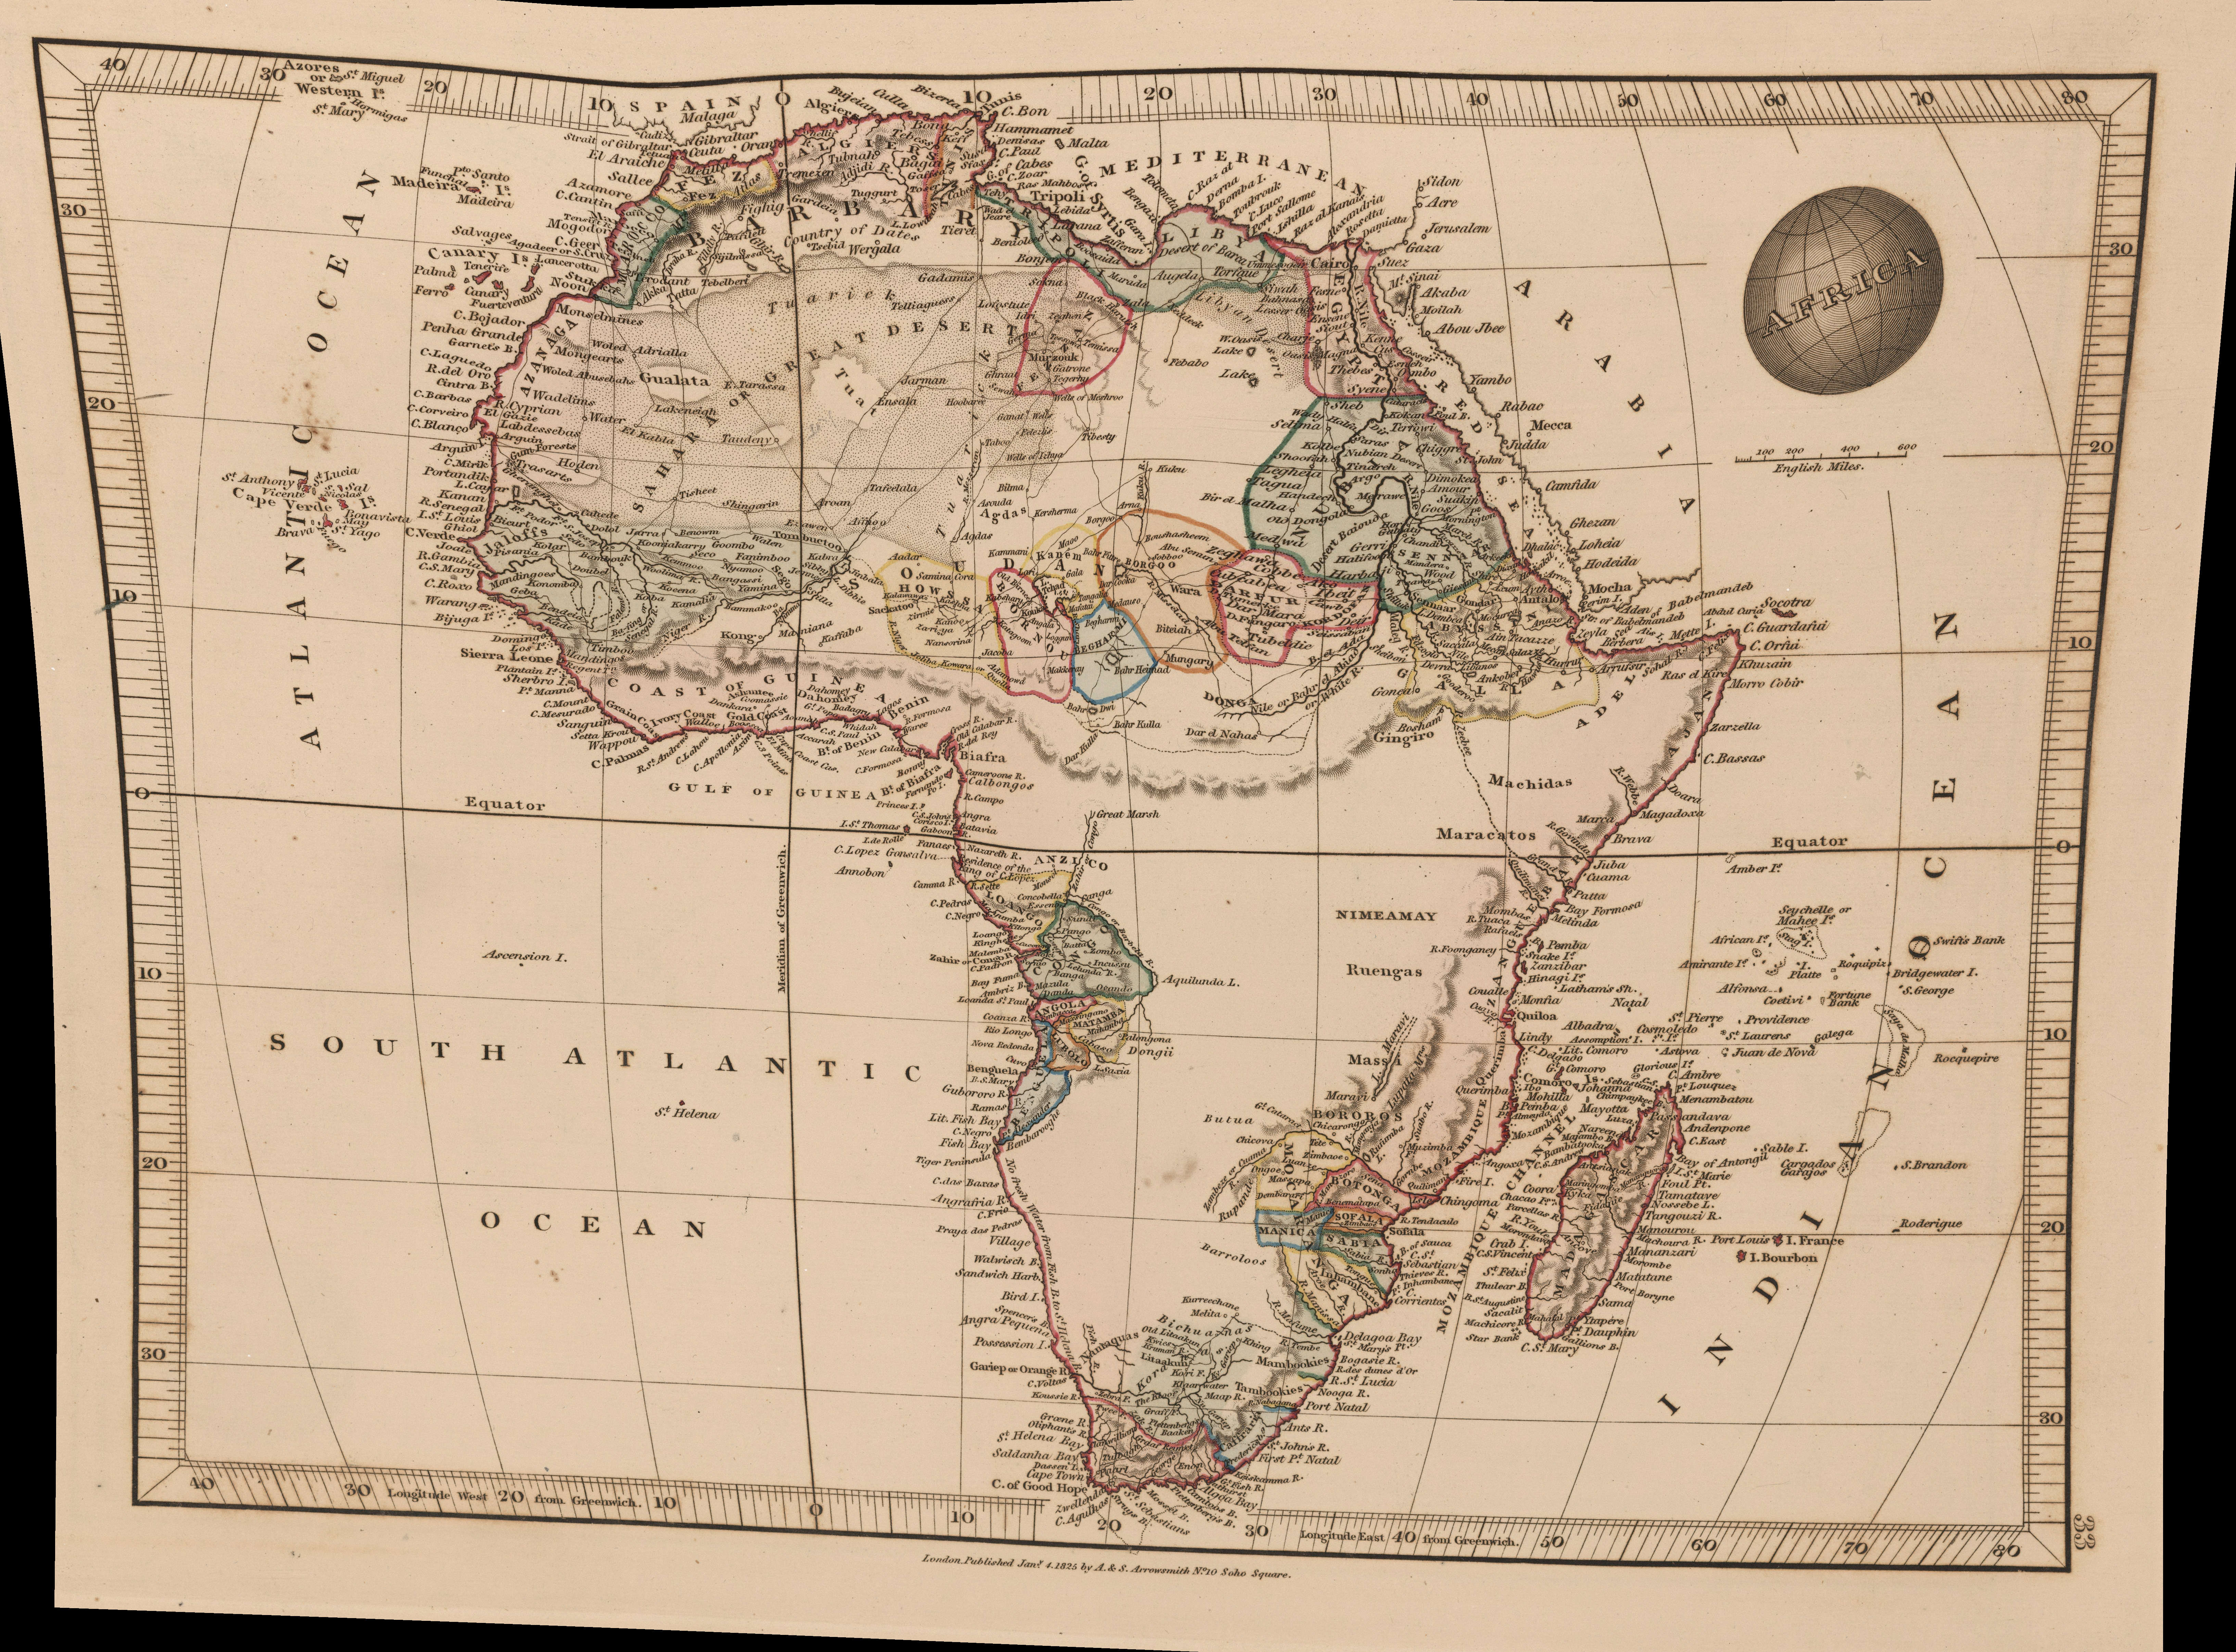
\includegraphics[width=0.8\linewidth]{img/Arrowsmith.jpg}
	\end{figure}

\end{frame}

\begin{frame}{Lots of old maps on top of each other}

	\begin{figure}[htpb]
		\centering
		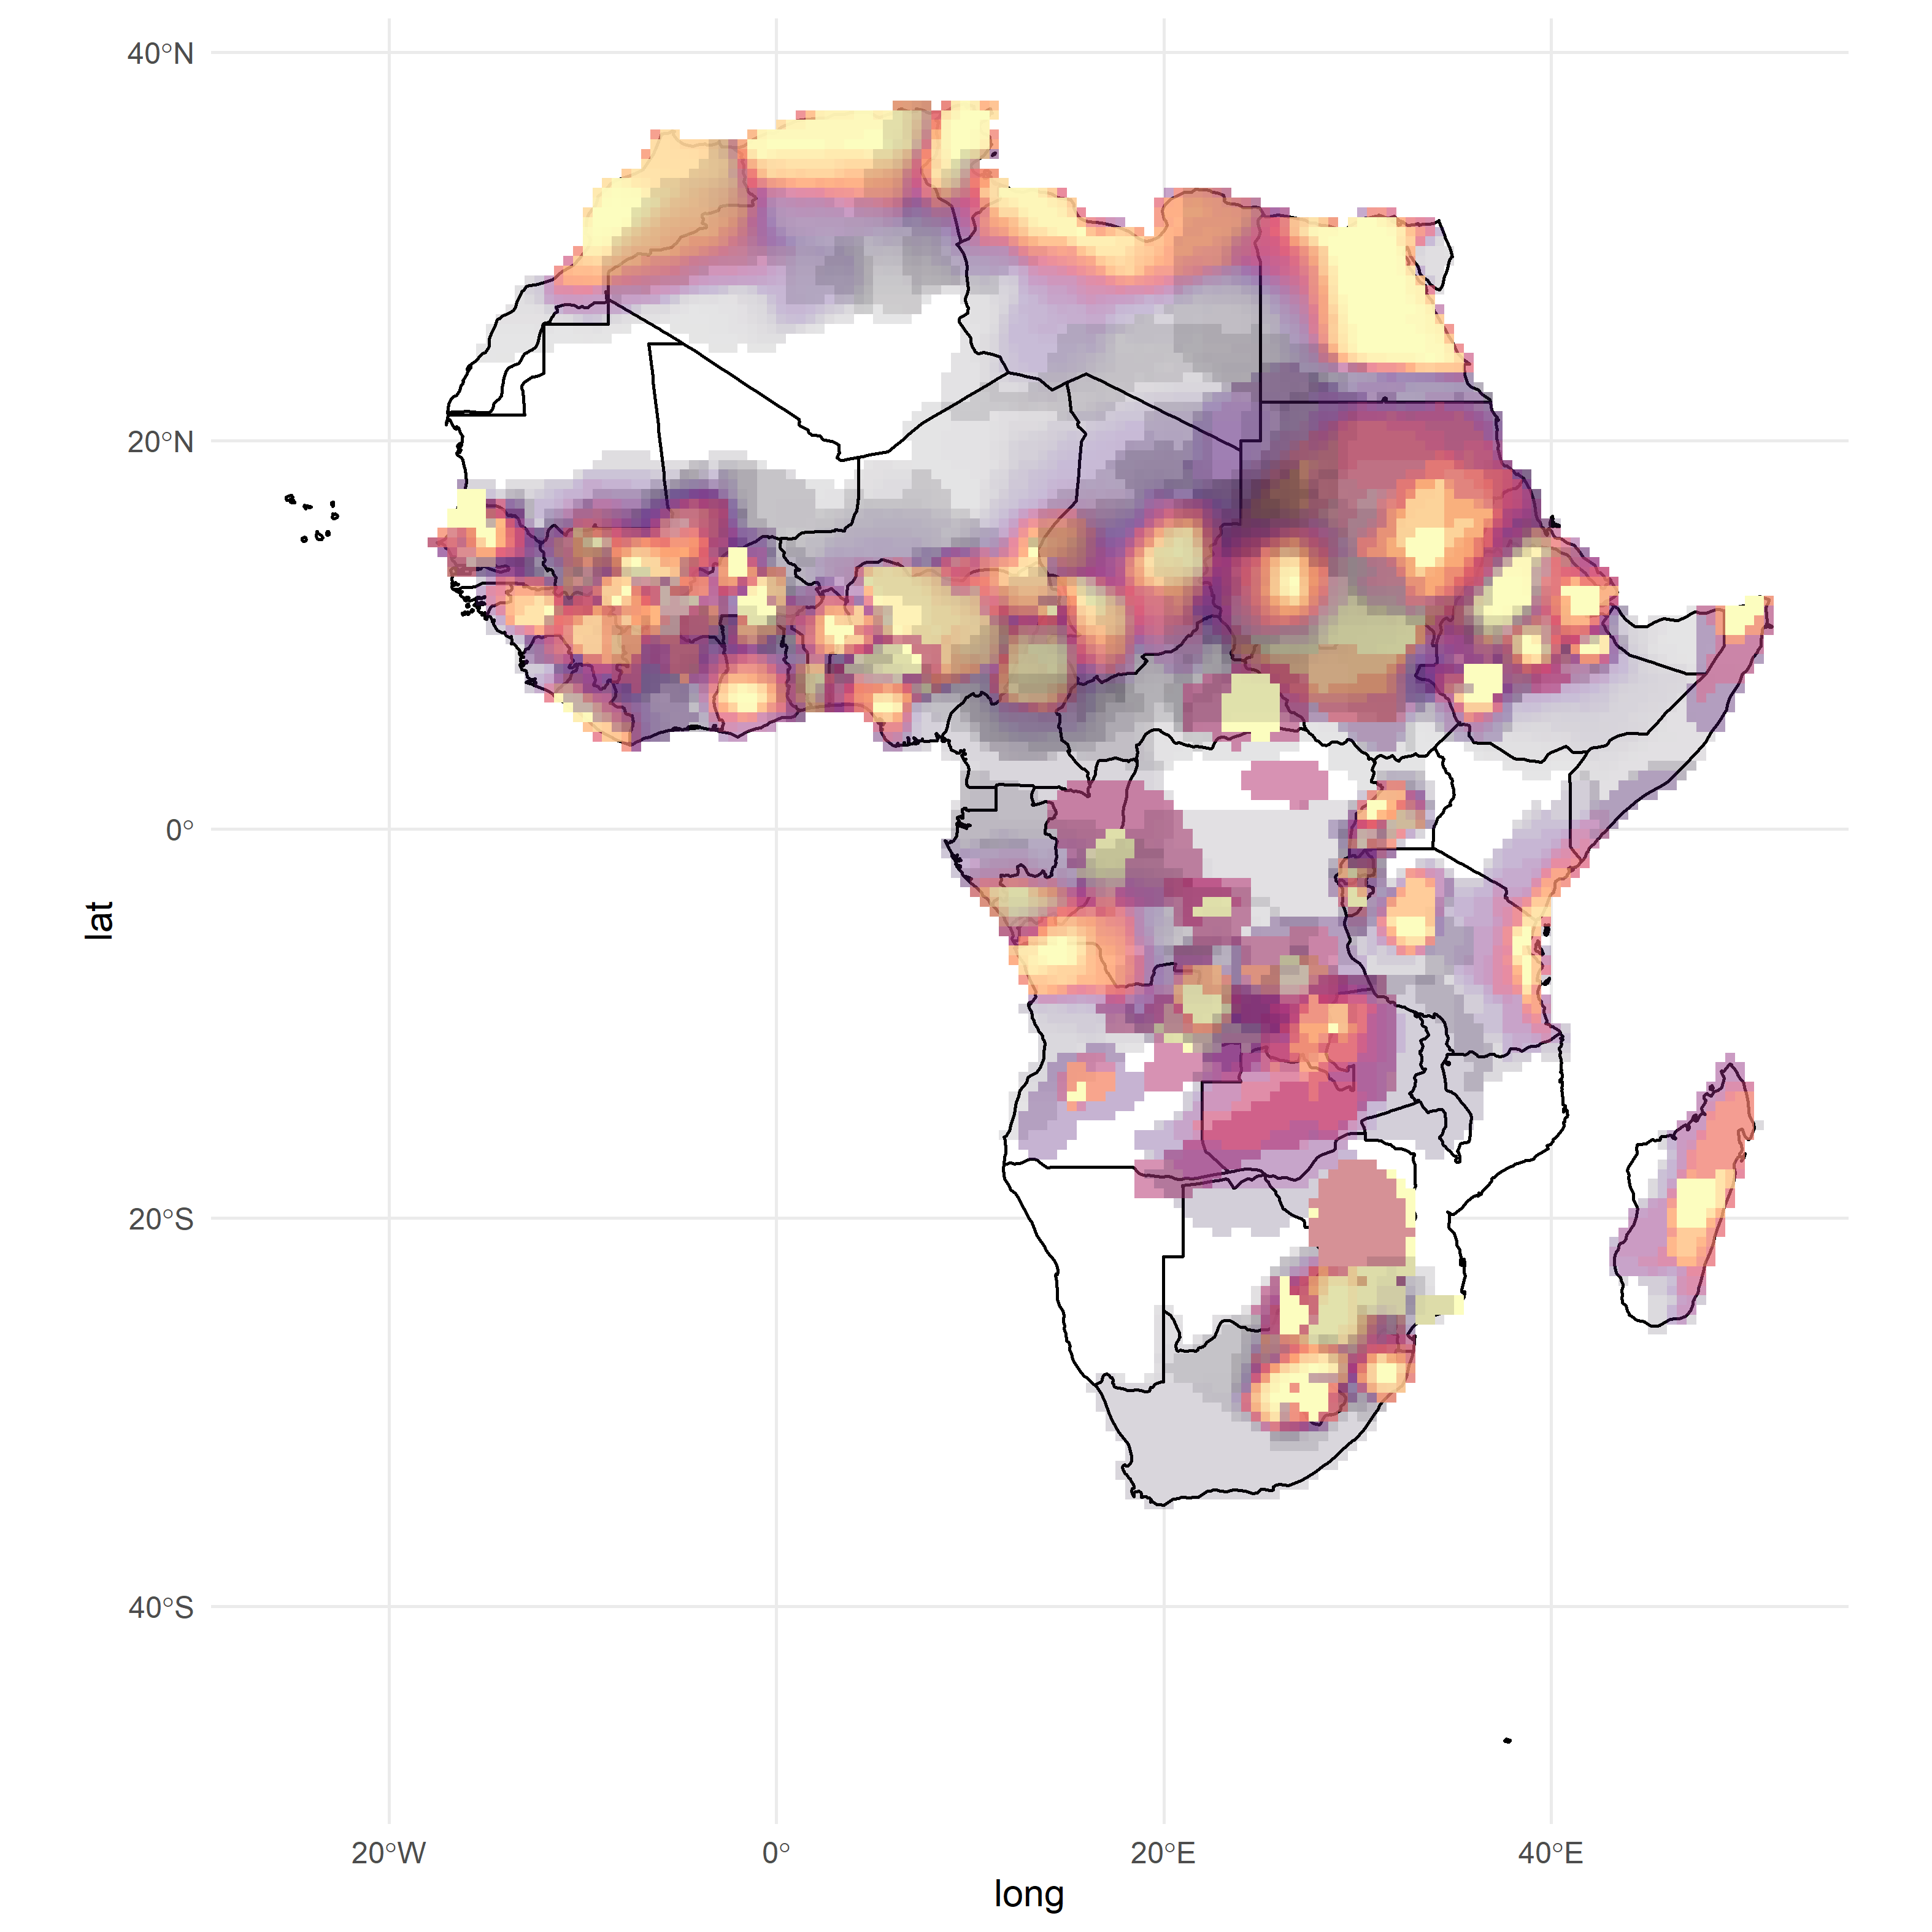
\includegraphics[width=0.7\linewidth]{img/geo_isd_all.png}
	\end{figure}

\end{frame}

\begin{frame}{Lots of old maps on top of each other}

	\begin{columns}

		\column{.5\textwidth}

		\begin{figure}[htpb]
			\centering
			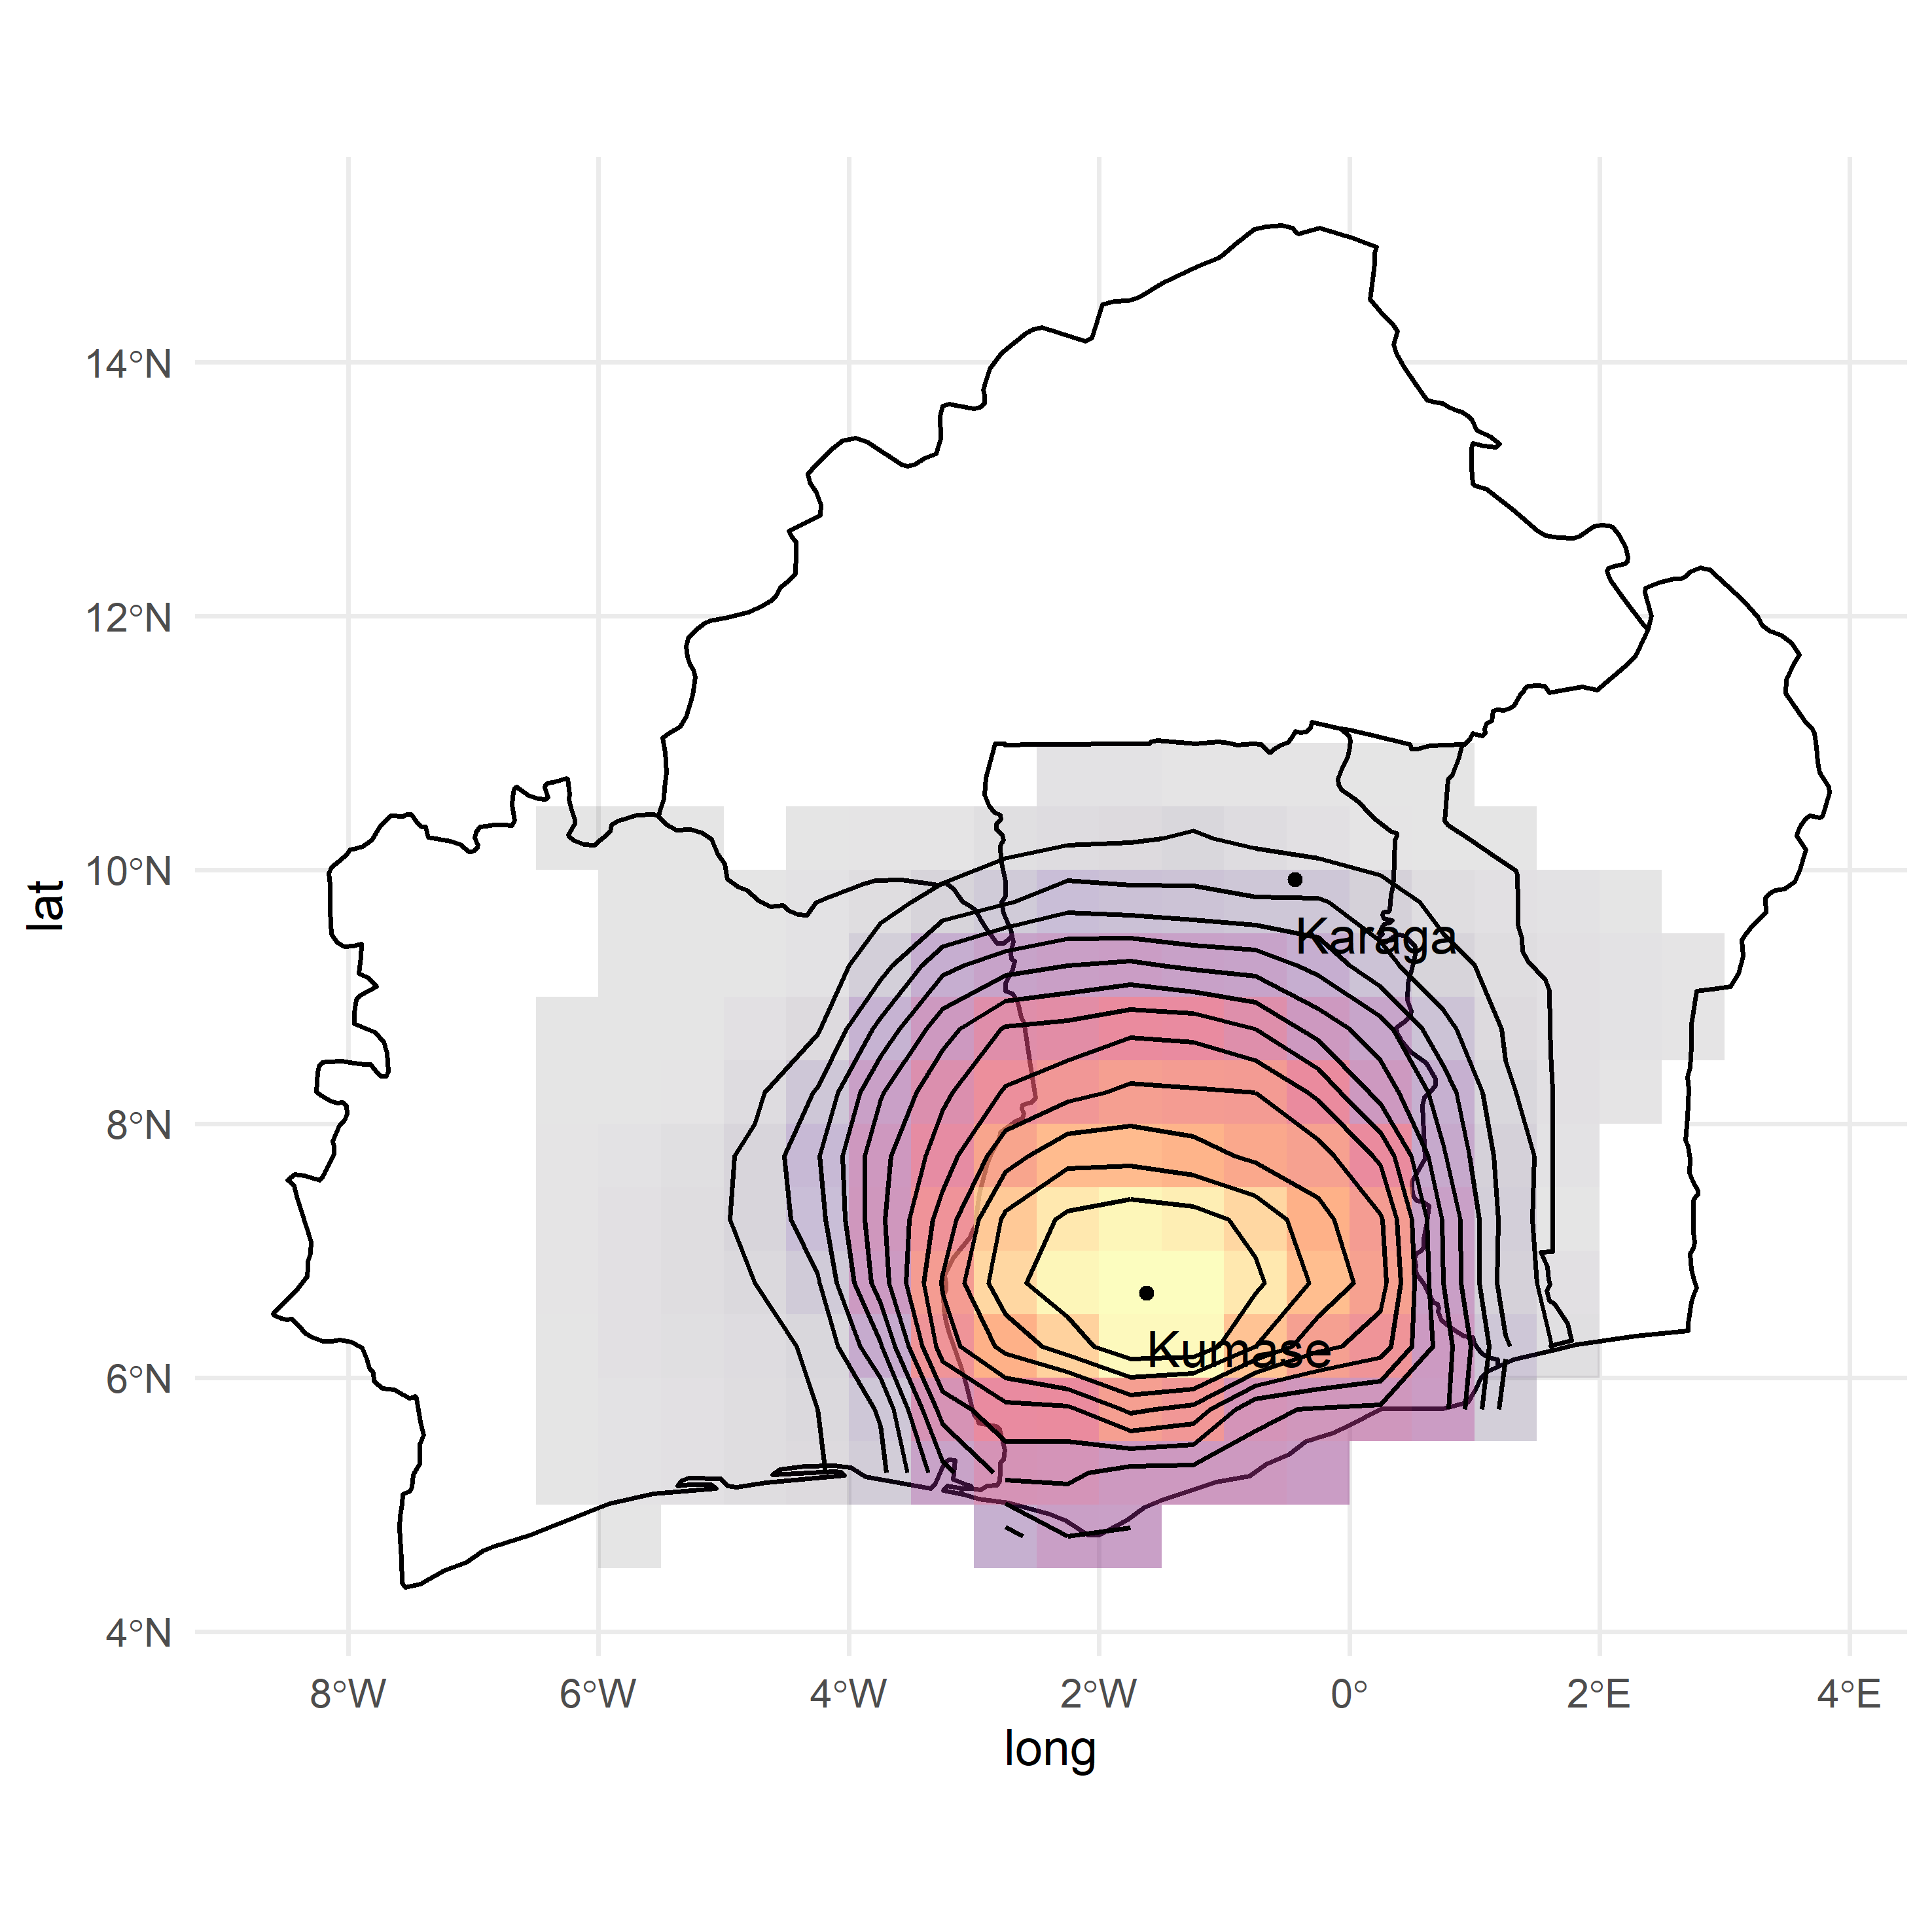
\includegraphics[width=0.8\linewidth]{img/asante.png}
			\caption{Asante}
		\end{figure}

		\column{.5\textwidth}

		\begin{figure}[htpb]
			\centering
			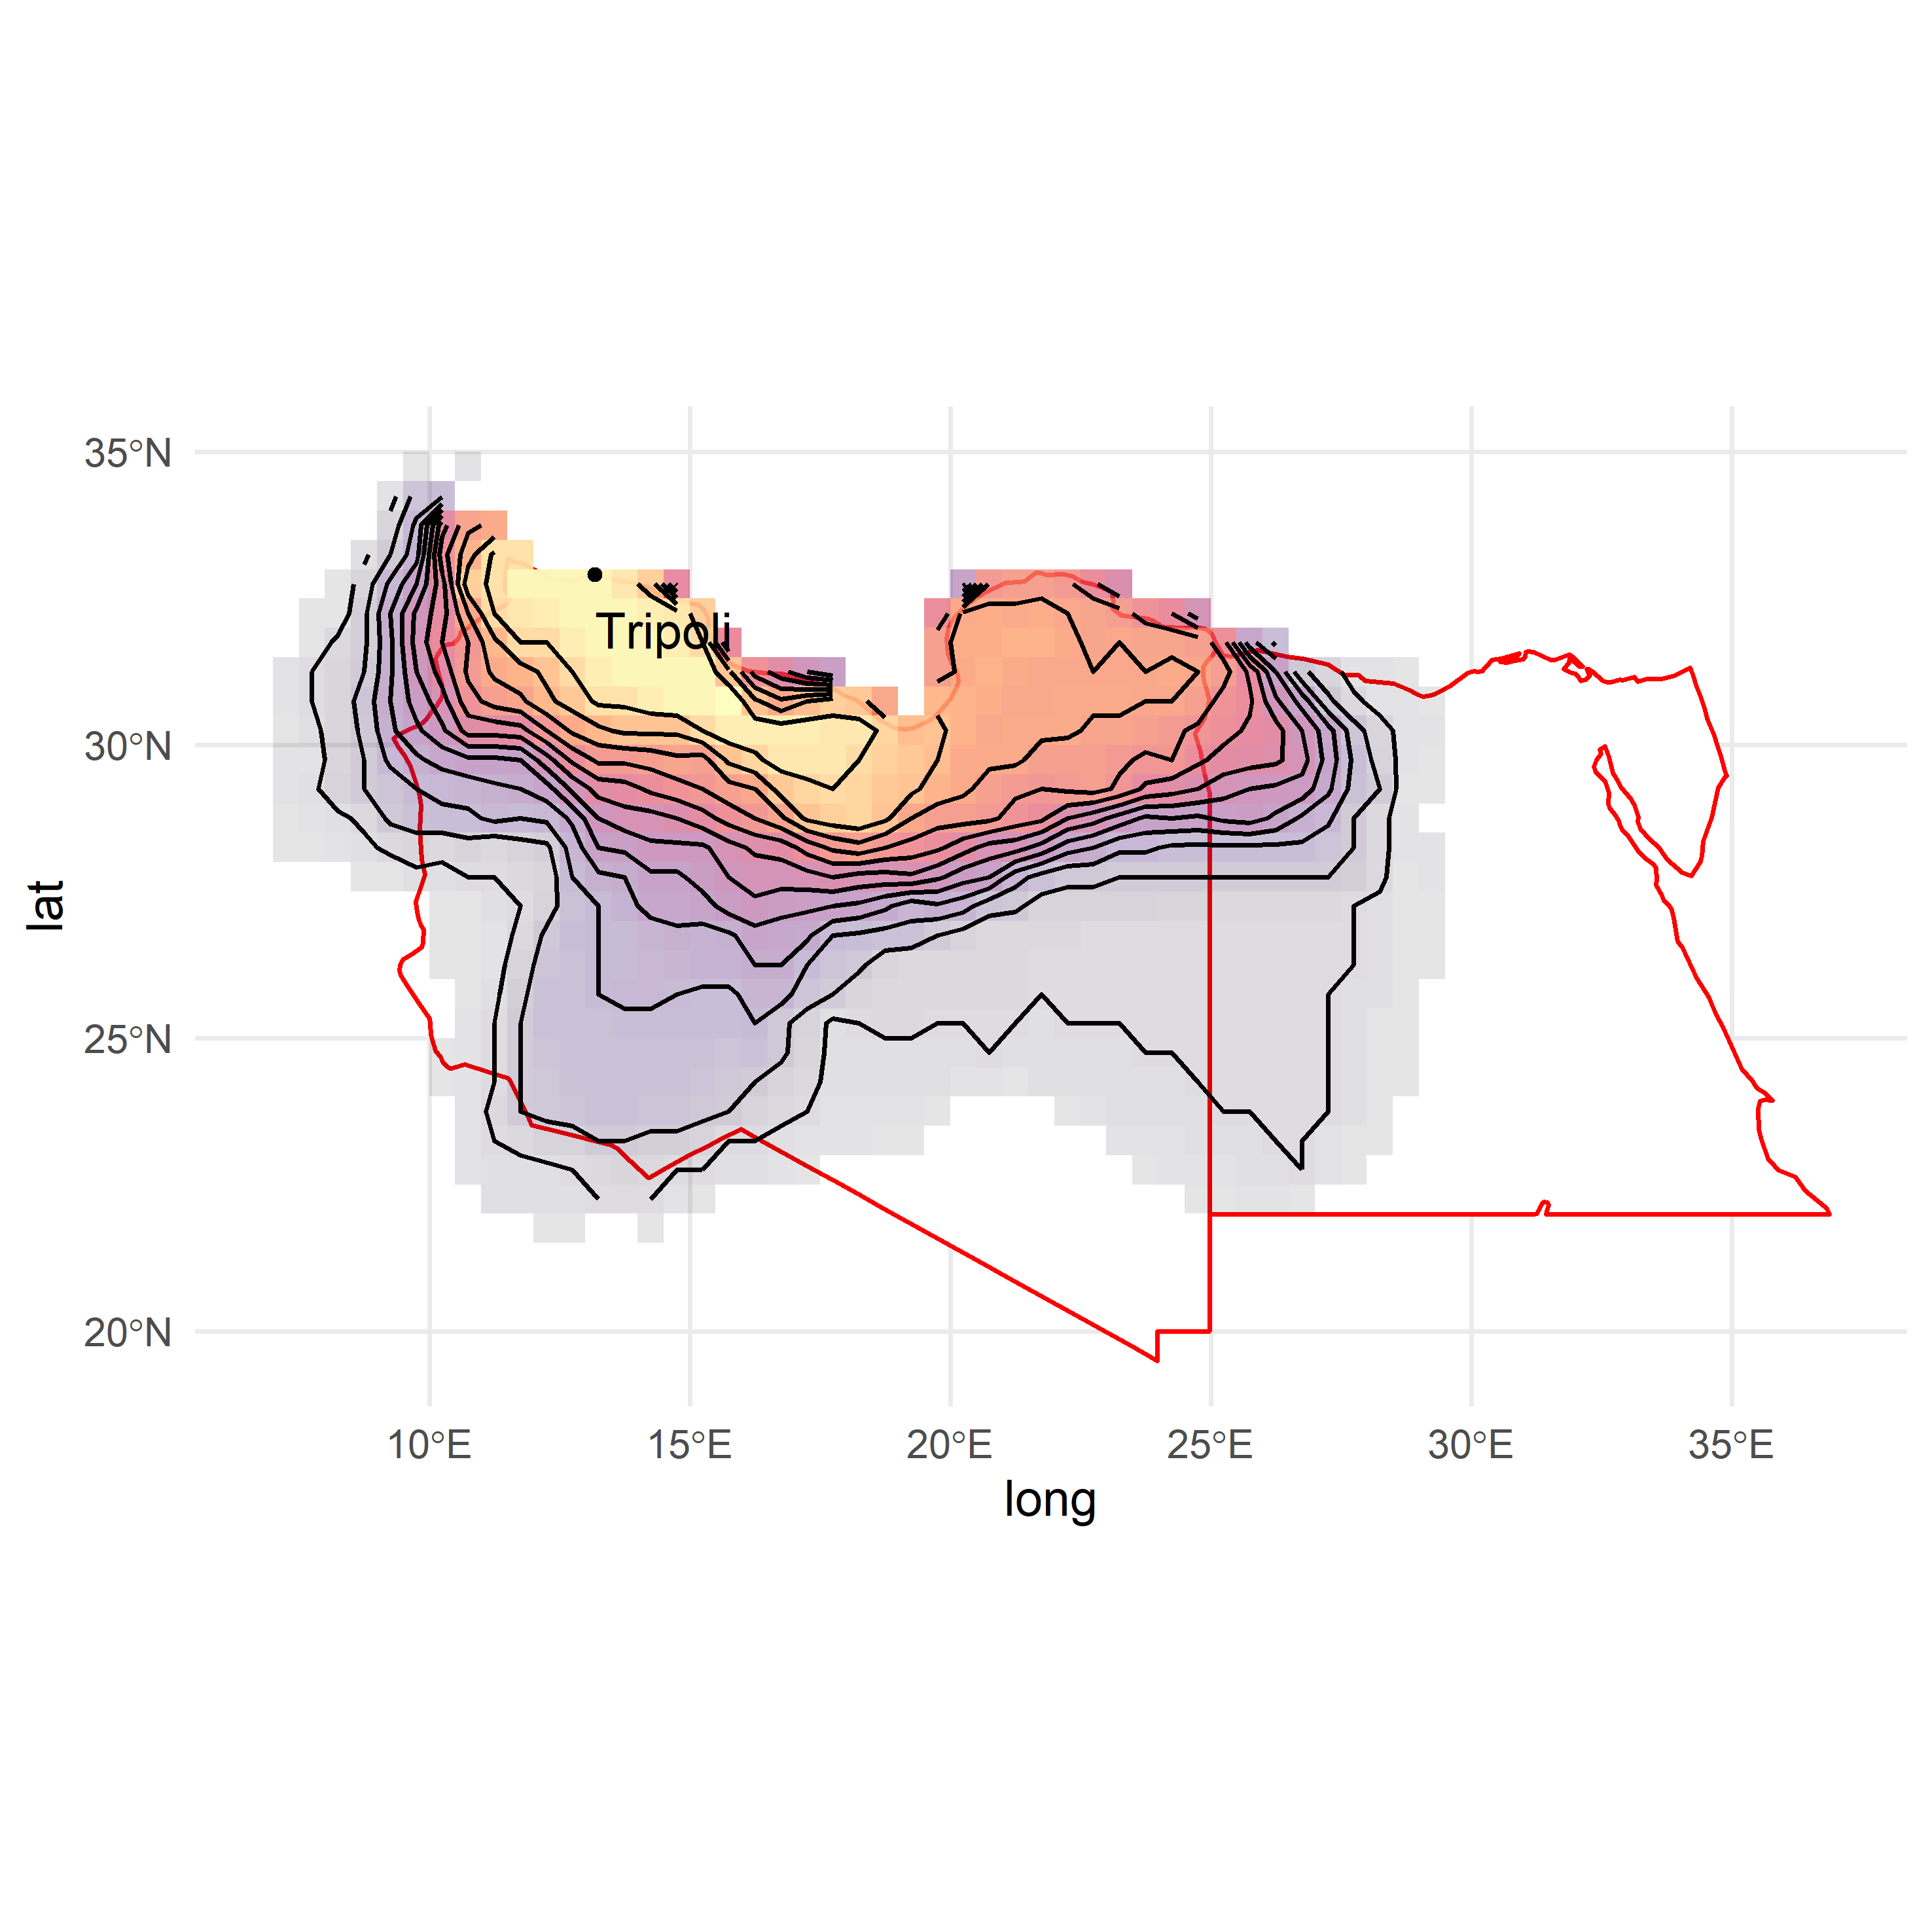
\includegraphics[width=0.8\linewidth]{img/libya.png}
			\caption{Libya}
		\end{figure}

	\end{columns}

\end{frame}

\begin{frame}{How accurate were these maps?}
		\begin{itemize}
			\item[-] Technically \pause % 36.9km
			\item[-] Drawing what they wanted to see?
		\end{itemize}
\end{frame}

\begin{frame}{How accurate were these maps?}

	\begin{figure}[htpb]
		\centering
		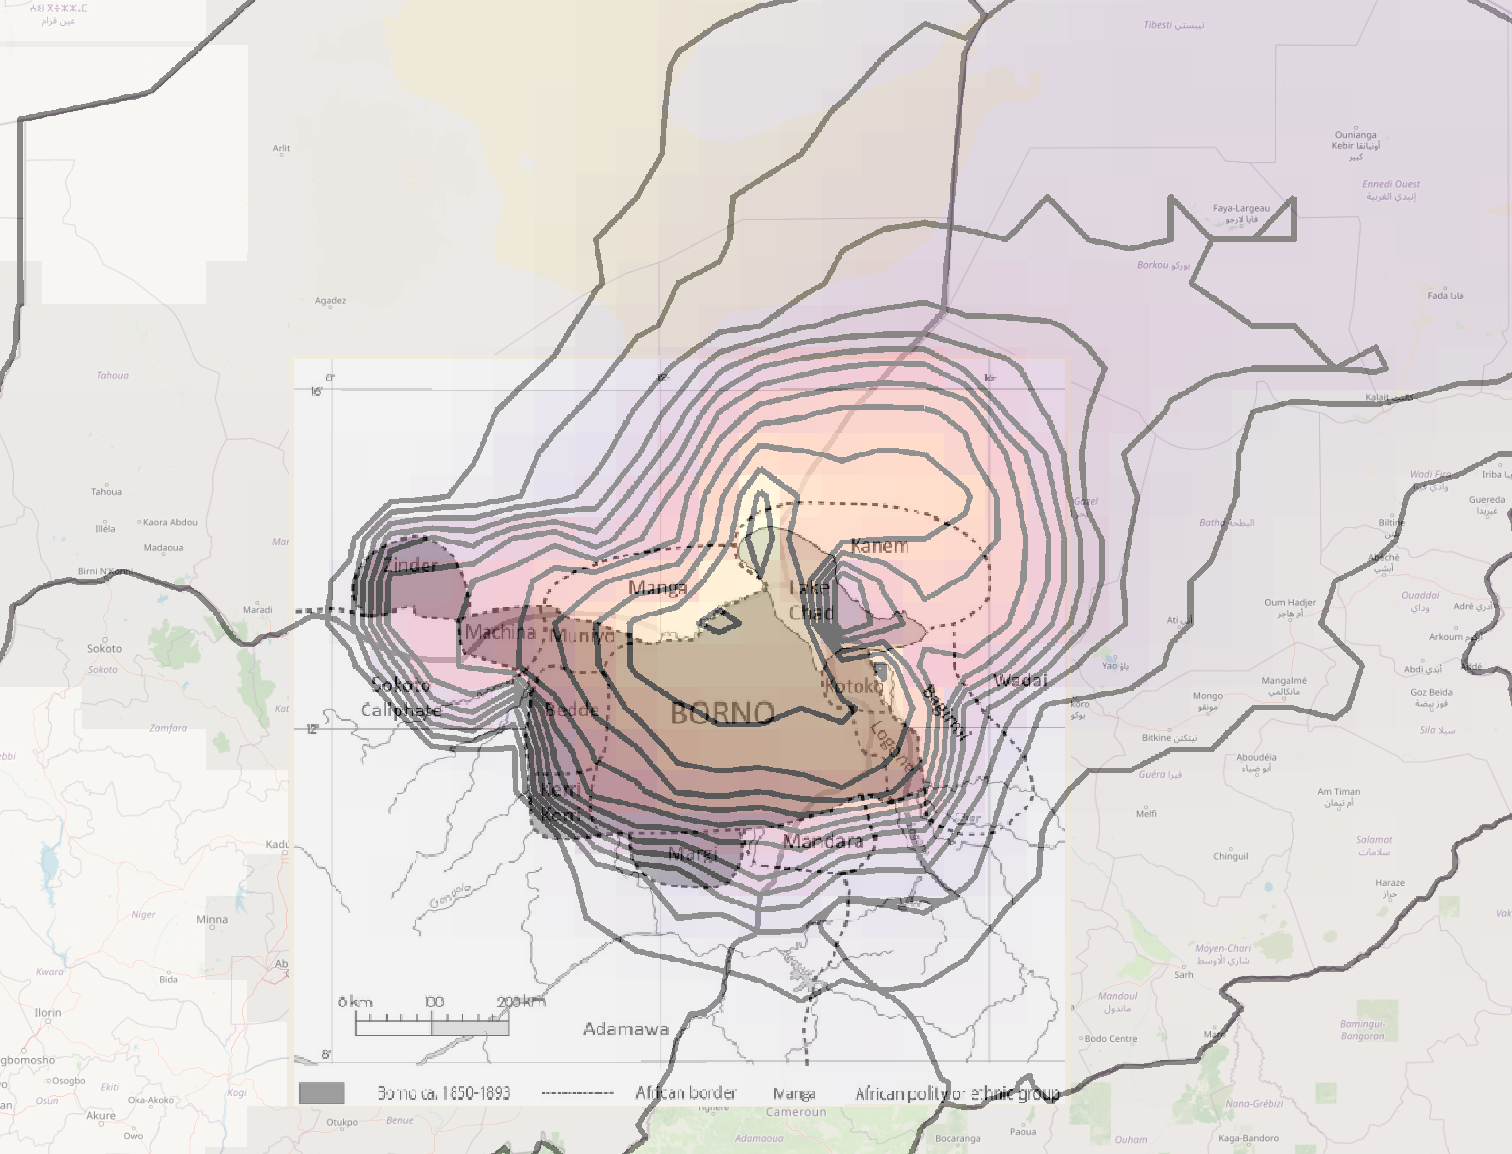
\includegraphics[width=0.8\linewidth]{img/kanem_bornu_hist.png}
		\caption{Kanem Bournu}
	\end{figure}

\end{frame}

% I now have a pretty good measure of where and to what degree these states have
% been present! 

\section{PCS's and civil conflict}

\begin{frame}{The big question}

Conflict inducing or conflict reducing?	

\end{frame}

\begin{frame}{Why not both?}

	\begin{figure}[htpb]
		\centering
		
\includegraphics[width=0.8\linewidth]{img/bothsides.jpg}
	\end{figure}

\end{frame}

\begin{frame}{The argument}

	Which mechanism dominates depends on how easy it is for the government
	to co-opt whatever is left of the pre-colonial states % As is determined by that states presence and
	% distance from capital

\end{frame}

\begin{frame}{Results}

	\begin{figure}[htpb]
		\centering
		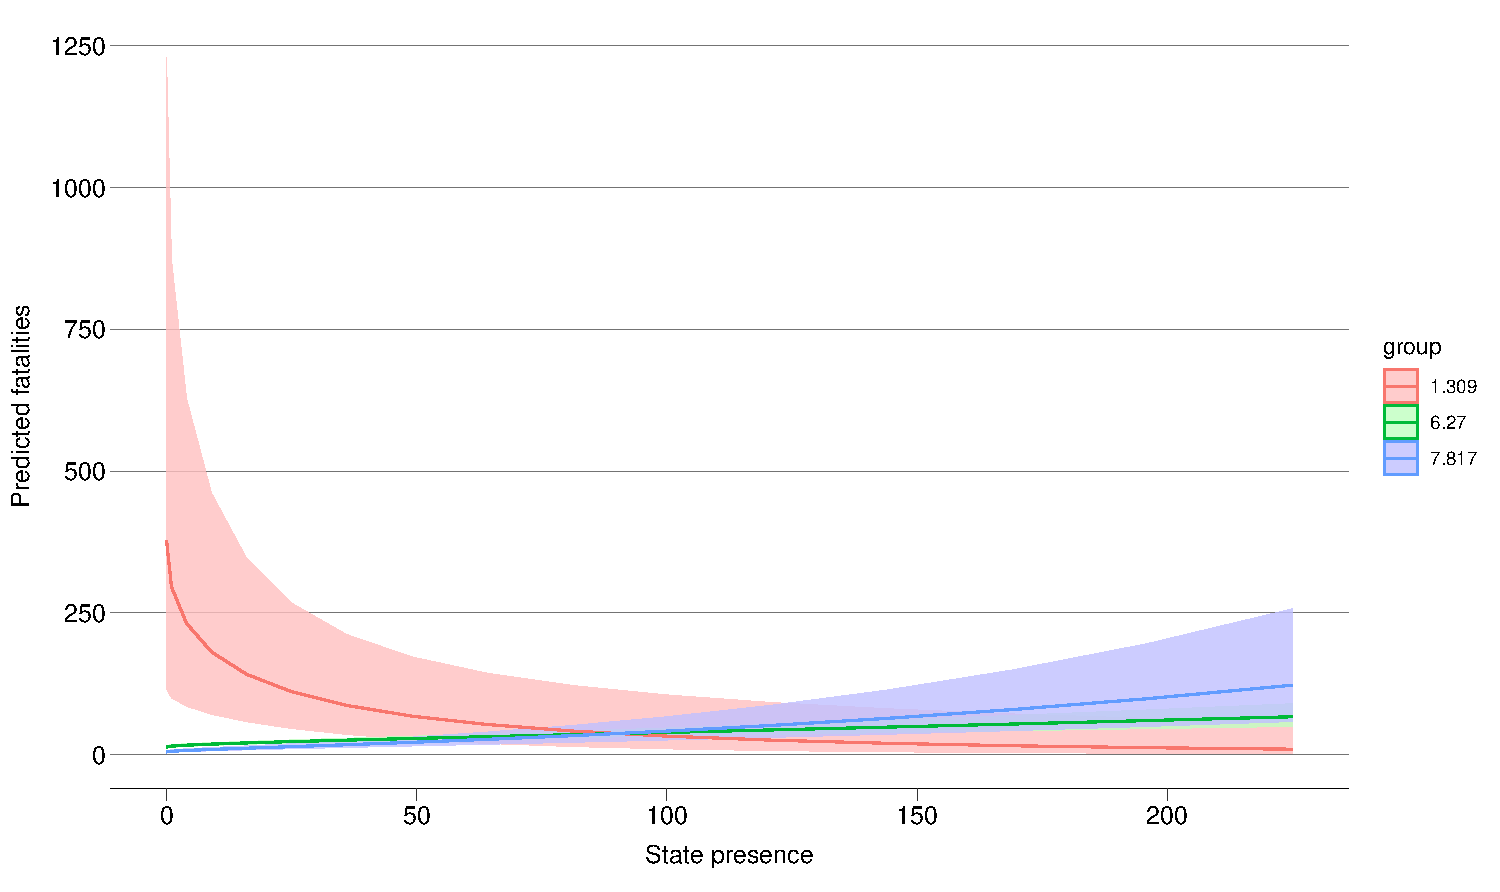
\includegraphics[width=0.8\linewidth]{../R/Output/deathsIntPlot.pdf}
	\end{figure}

\end{frame}

\begin{frame}{References}

\small{
\bibliographystyle{agsm}
\bibliography{../lib.bib}
}

\end{frame}

\end{document}
